\begin{center}
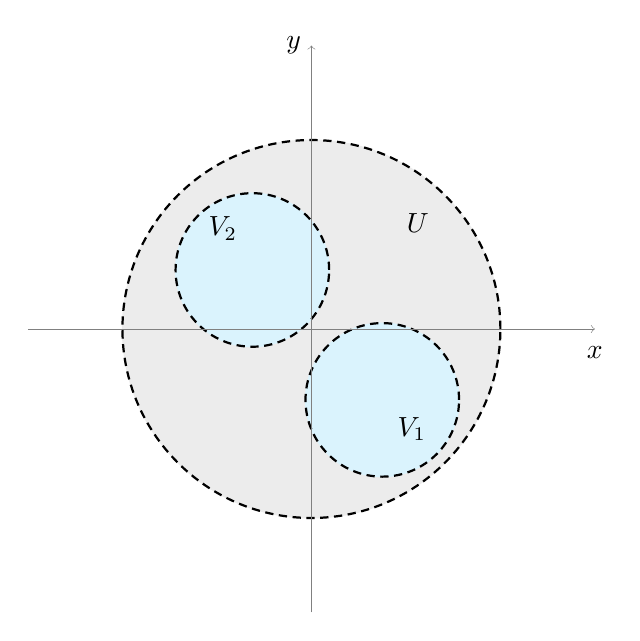
\begin{tikzpicture}[scale = 0.75]
\def\gap{0.2}
\def\bigradius{3.2}
\def\smallradius{1.3}


\filldraw[gray!15] (0,0) circle (\bigradius cm);
\draw[thick, densely dashed] (0,0) circle (\bigradius cm);

\filldraw[ProcessBlue!15] (-1,1) circle (\smallradius cm);
\draw[thick, densely dashed] (-1,1) circle (\smallradius cm);

\filldraw[ProcessBlue!15] (1.2,-1.2) circle (\smallradius cm);
\draw[thick, densely dashed] (1.2,-1.2) circle (\smallradius cm);


\draw [help lines,->] (-1.5*\bigradius, 0) -- (1.5*\bigradius,0);
\draw [help lines,->] (0, -1.5*\bigradius) -- (0,1.5*\bigradius);

\node at (1.5*\bigradius,-0.4){$x$};
\node at (-0.3, 1.5*\bigradius) {$y$};

\node at (1.8, 1.8) {$U$};
\node at (1.7, -1.7) {$V_1$};
\node at (-1.5, 1.7) {$V_2$};

\end{tikzpicture}
\begin{tikzpicture}[scale = 0.75]
\def\gap{0.2}
\def\bigradius{3.2}
\def\smallradius{1.3}


\filldraw[gray!15] (0,0) circle (\bigradius cm);
\draw[thick, densely dashed] (0,0) circle (\bigradius cm);







\begin{scope}[scale = 0.74]
\filldraw[ProcessBlue!15] plot[smooth, tension=.7, closed hobby] coordinates {
(-2.1,1.5) (-1,2.5) (1.5,1) (4,0.5) (3,-0.5) (2.5,-3)
(0,-0.2) (-3,-2.5)};
\draw[densely dashed, thick] plot[smooth, tension=.7, closed hobby] coordinates {
(-2.1,1.5) (-1,2.5) (1.5,1) (4,0.5) (3,-0.5) (2.5,-3)
(0,-0.2) (-3,-2.5)};
\end{scope}


\draw [help lines,->] (-1.5*\bigradius, 0) -- (1.5*\bigradius,0);
\draw [help lines,->] (0, -1.5*\bigradius) -- (0,1.5*\bigradius);

\node at (1.5*\bigradius,-0.4){$x$};
\node at (-0.3, 1.5*\bigradius) {$y$};

\node at (1.8, 1.8) {$U$};
\node at (-2.1, -1.4) {$V$};
\end{tikzpicture}        
\end{center}